\chapter{Metodologia}
\label{cap:metodologia}

\section{Caracterização da pesquisa}
\label{sec:caracterizacao}

Quanto à abordagem, a pesquisa é \textbf{quantitativa}: as hipóteses formuladas
na Seção~\ref{sec:hipoteses} são testadas por comparação de métricas numéricas de
erro sob protocolo experimental controlado, com quantificação de incerteza por
reamostragem. Quanto aos objetivos, é \textbf{explicativa}, pois busca
estabelecer relação causal entre a introdução de restrições físicas na função de
perda e a variação observada no erro de generalização, mantendo controladas as
demais condições experimentais. Quanto aos procedimentos, combina pesquisa
\textbf{bibliográfica}, na construção do referencial teórico e no levantamento do
estado da arte, e pesquisa \textbf{experimental}, na condução dos experimentos
computacionais sobre base de dados secundária de acesso público.

O objeto de estudo é constituído por dados simulados, não por medições
experimentais próprias. Essa escolha é deliberada e responde a uma limitação
concreta: o escâner tridimensional de campo próximo desenvolvido pelo autor em
iniciação científica encontra-se em fase de desenvolvimento e não fornece, no
momento, medições com incerteza caracterizada. O uso de base simulada e validada
por terceiros elimina essa fonte de risco do caminho crítico do trabalho,
preservando o escâner como instrumento de validação qualitativa complementar,
conforme detalhado na Seção~\ref{sec:validacao_exp}.

\section{Base de dados}
\label{sec:dados}

\subsection{Origem e licenciamento}

Utiliza-se a SI/PI-Database, mantida pelo \textit{Institut für Theoretische
Elektrotechnik} da Universidade Técnica de Hamburgo \citep{schierholz2021,
hillebrecht2024}. O acesso é público mediante preenchimento de formulário e
aceite dos termos de uso, que exigem a citação dos artigos de referência em
qualquer publicação derivada. Os dados foram obtidos e encontram-se armazenados
localmente.

\subsection{Subconjunto principal}

O subconjunto adotado como objeto principal é o \textit{6-Layer PCB based PDN
with Two Via Arrays}, amostrado por hipercubo latino. Sua caracterização, obtida
por inspeção direta dos arquivos, está resumida na
Tabela~\ref{tab:dataset}.

\begin{table}[htb]
\centering
\caption{Caracterização do subconjunto principal de dados}
\label{tab:dataset}
\footnotesize
\begin{tabular}{@{}ll@{}}
\toprule
\textbf{Atributo} & \textbf{Valor verificado} \\
\midrule
Número de configurações & 985 \\
Volume descompactado & 24{,}0\,GB \\
Formato da resposta & Touchstone v1.1, \texttt{.s36p}, real--imaginário \\
Número de portas & 36 \\
Pontos de frequência & 334 \\
Faixa de frequência & 1\,MHz a 1\,GHz \\
Espaçamento em frequência & linear, passo de 3\,MHz \\
Parâmetros no arquivo tabular & 17 (mais o índice de simulação) \\
Parâmetros efetivamente variados & 8 \\
\bottomrule
\end{tabular}
\vspace{0.3em}
\\{\footnotesize FONTE: O autor (2026), por inspeção direta dos arquivos.}
\end{table}

A distinção entre parâmetros presentes e parâmetros efetivamente variados é
metodologicamente relevante e foi estabelecida por análise de cardinalidade de
cada coluna. Dos dezessete parâmetros do arquivo tabular, nove permanecem
constantes em todas as 985 configurações: espessura de metalização
($1$\,mil), dimensões laterais da placa ($5800 \times 4000$\,mil), condutividade
($5{,}8\times 10^7$\,S/m), tangente de perdas ($0{,}01$) e as coordenadas dos
centros dos dois arranjos de vias. Restam oito graus de liberdade efetivos,
relacionados na Tabela~\ref{tab:features}.

\begin{table}[htb]
\centering
\caption{Parâmetros efetivamente variados e respectivas faixas}
\label{tab:features}
\footnotesize
\begin{tabular}{@{}llrrr@{}}
\toprule
\textbf{Parâmetro} & \textbf{Grandeza física} & \textbf{Mínimo} &
\textbf{Máximo} & \textbf{Níveis} \\
\midrule
\texttt{TDIEL} & espessura do dielétrico & 3{,}12 & 78{,}99 & 984 \\
\texttt{PERMITTIVITY} & permissividade relativa $\varepsilon_r$ & 2{,}50 &
4{,}50 & 984 \\
\texttt{A1\_VIARADIUS} & raio da via, arranjo 1 & 10 & 20 & 11 \\
\texttt{A1\_ANTIPADRADIUS} & raio do \textit{antipad}, arranjo 1 & 20 & 39 &
20 \\
\texttt{A1\_VIAPITCH} & passo do arranjo 1 & 80 & 120 & 9 \\
\texttt{A2\_VIARADIUS} & raio da via, arranjo 2 & 10 & 20 & 11 \\
\texttt{A2\_ANTIPADRADIUS} & raio do \textit{antipad}, arranjo 2 & 20 & 39 &
20 \\
\texttt{A2\_VIAPITCH} & passo do arranjo 2 & 80 & 120 & 9 \\
\bottomrule
\end{tabular}
\vspace{0.3em}
\\{\footnotesize NOTA: dimensões geométricas em mil ($1$\,mil $= 25{,}4\,\mu$m),
sujeitas à confirmação descrita na Seção~\ref{subsec:riscos_dados}.
\\FONTE: O autor (2026), por inspeção direta de \texttt{parameter.csv}.}
\end{table}

Esse achado corrige uma premissa inicial do projeto, que assumia treze variáveis
de entrada, e tem duas consequências diretas. A primeira é favorável: um espaço
de projeto de oito dimensões amostrado por hipercubo latino com 985 pontos
apresenta densidade amostral razoável, o que torna o problema tratável. A
segunda impõe cautela na formulação das conclusões, pois parâmetros como
condutividade e tangente de perdas, mantidos fixos, não poderão ter seu efeito
estimado, e qualquer diretriz de projeto derivada estará condicionada aos valores
adotados na geração da base.

\subsection{Subconjuntos secundários}

Os subconjuntos \textit{Universal SE-SI Array} (1932 configurações) e
\textit{Universal Diff-SI Array} (1916 configurações), também já obtidos, cobrem
espaço de projeto substancialmente mais rico — quatorze parâmetros variados,
número de camadas entre 4 e 48, e faixa de 250\,MHz a 100\,GHz. Eles apresentam,
contudo, uma dificuldade estrutural: o número de portas varia entre configurações
(de 6 a 58), de modo que a dimensão da matriz de resposta não é constante ao
longo da base. Isso inviabiliza o uso de arquiteturas de entrada e saída fixas
sem uma etapa adicional de agregação ou de modelagem por conjuntos. Por essa
razão, esses subconjuntos são reservados como extensão opcional, condicionada ao
cumprimento antecipado dos marcos principais, e não integram o caminho crítico.

\subsection{Riscos associados aos dados e sua mitigação}
\label{subsec:riscos_dados}

Três riscos foram identificados na etapa de caracterização e serão tratados
antes do início da modelagem.

\begin{alineas}
\item \textbf{Ambiguidade de unidades.} A documentação não declara
explicitamente as unidades das dimensões geométricas. A hipótese de que estejam
em mil é sustentada por dois indícios convergentes: $5800 \times 4000$\,mil
corresponde a $147{,}3 \times 101{,}6$\,mm, praticamente coincidente com o
formato Eurocard padrão de $160 \times 100$\,mm; e, sob essa hipótese, a
capacitância extraída da resposta simulada situa-se na faixa de 0{,}5 a 8\,nF
(Seção~\ref{sec:preliminar}), com mediana cerca de duas vezes a previsão de
cavidade única — compatível com uma porta acoplada a duas cavidades em paralelo
em um empilhamento de seis camadas. A hipótese alternativa, de dimensões em
micrômetro, implicaria capacitância extraída uma ordem de grandeza \emph{abaixo}
da de uma única cavidade, o que é fisicamente inadmissível. A confirmação
definitiva será obtida junto aos mantenedores da base;

\item \textbf{Subamostragem da primeira década.} O espaçamento em frequência é
linear com passo de 3\,MHz, o que aloca apenas quatro pontos à década de 1 a
10\,MHz e mais de trezentos à década de 100\,MHz a 1\,GHz. Como o comportamento
capacitivo de baixa frequência é justamente o ancoradouro de uma das restrições
físicas propostas, a métrica de erro será ponderada por década, evitando que o
desempenho na região de alta frequência domine a função objetivo e mascare erros
na região capacitiva;

\item \textbf{Volume de dados.} Cada arquivo Touchstone ocupa aproximadamente
24\,MB e contém a matriz completa de $36 \times 36$ portas, dos quais apenas um
subconjunto reduzido de colunas é necessário. Será implementada uma etapa de
pré-processamento que extrai as grandezas de interesse e as persiste em formato
colunar comprimido, reduzindo o volume em cerca de duas ordens de grandeza e
tornando o conjunto residente em memória durante o treinamento.
\end{alineas}

\section{Definição do alvo de predição}
\label{sec:alvo}

O alvo primário é a curva de autoimpedância $|Z_{11}(f)| \in \mathbb{R}^{334}$,
obtida da matriz de espalhamento pela Equação~\ref{eq:s2z}. Prediz-se a curva
completa, e não apenas um escalar agregado, por duas razões. Primeira, a curva é
o que o projetista efetivamente precisa para confrontar com a impedância-alvo da
Equação~\ref{eq:ztarget}. Segunda, e mais importante para o desenho experimental,
as restrições físicas propostas incidem sobre a forma da curva — seu
comportamento assintótico e a localização de seus máximos — e seriam inexprimíveis
sobre um alvo escalar.

Adota-se a representação $y(f) = \log_{10}|Z_{11}(f)|$, pela qual a impedância
varre várias ordens de grandeza ao longo da faixa. A transformação logarítmica
uniformiza a escala do erro, alinha a métrica de otimização com a percepção de
engenharia — que raciocina em decibéis — e converte o comportamento capacitivo de
baixa frequência em uma reta, o que simplifica a formulação do termo de perda
correspondente.

Como métricas secundárias, derivadas da curva predita, registram-se
$|Z|_{\max}$ e a frequência em que ocorre, por serem os indicadores diretamente
associados ao risco de emissão irradiada.

\section{Investigação preliminar das âncoras físicas}
\label{sec:preliminar}

Antes de fixar a formulação dos termos de perda, conduziu-se uma investigação
preliminar destinada a verificar, sobre os próprios dados, quais das relações
analíticas da Seção~\ref{sec:pdn} são de fato observáveis na grandeza a ser
predita. O procedimento consistiu em extrair $Z_{11}(f)$ de uma amostra aleatória
de 40 configurações, com semente registrada, e confrontar o resultado com as
previsões das Equações~\ref{eq:modos} e~\ref{eq:cplate}. Os resultados estão
sintetizados na Figura~\ref{fig:ancoras}.

\begin{figure}[htb]
\centering
\caption{Verificação preliminar das âncoras físicas sobre o conjunto de dados}
\label{fig:ancoras}
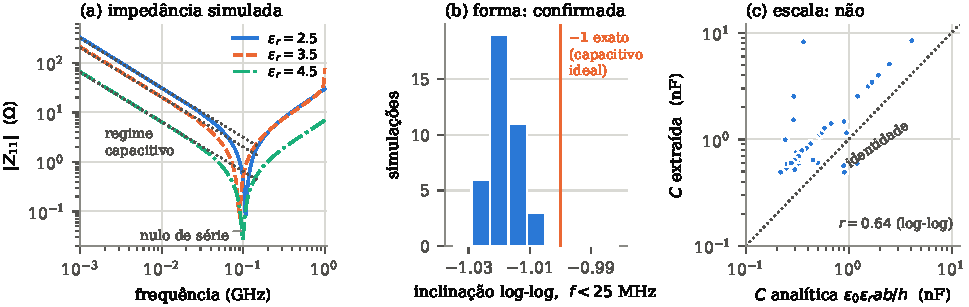
\includegraphics[width=\linewidth]{3-metodo/figuras/ancoras_fisicas.pdf}
\vspace{0.2em}
\\{\footnotesize NOTA: (a) curvas de $|Z_{11}|$ para três configurações de
permissividade contrastante, com a assíntota capacitiva ajustada em linha
pontilhada; (b) distribuição da inclinação log-log abaixo de 25\,MHz em 40
configurações; (c) capacitância extraída da resposta simulada contra a previsão
de placas paralelas.
\\FONTE: O autor (2026).}
\end{figure}

Três achados orientam a formulação adotada.

\begin{alineas}
\item \textbf{A forma do regime capacitivo é confirmada com precisão.} A
inclinação log-log de $|Z_{11}|$ abaixo de 25\,MHz vale $-1{,}018 \pm 0{,}008$
nas 40 configurações analisadas, contra $-1$ para um capacitor ideal. O
comportamento quase-estático previsto pela Equação~\ref{eq:cplate} é, portanto,
uma descrição fiel da resposta nessa região;

\item \textbf{A escala absoluta da capacitância não é.} A capacitância extraída
da resposta simulada correlaciona-se com a previsão de placas paralelas
($r = 0{,}64$ em escala logarítmica), mas a razão entre ambas varia de $0{,}5$ a
mais de 20. O desvio é compatível com a estrutura de seis camadas, em que a
porta acopla-se a um número variável de cavidades em paralelo, efeito que a
fórmula de uma única cavidade não captura;

\item \textbf{Os modos de cavidade não são diretamente observáveis em
$Z_{11}$.} Ao contrário do que a Equação~\ref{eq:modos} levaria a supor, a
resposta não apresenta máximos pronunciados nas frequências modais dentro da
faixa analisada. A curva exibe, em vez disso, um nulo de série em torno de
100\,MHz, seguido de crescimento monotônico até o limite superior da banda. A
densidade de arranjos de vias amortece fortemente os modos, e a autoimpedância
em uma única porta não os evidencia.
\end{alineas}

O terceiro achado merece registro explícito porque contraria a expectativa
inicial deste projeto, que previa a localização modal como âncora física
principal. Uma verificação anterior, baseada em detecção de máximos locais,
havia sugerido concordância entre picos e modos previstos; inspeção gráfica
revelou que os máximos detectados eram ondulações numéricas de amplitude
desprezível e que, dada a densidade do espectro modal na faixa, qualquer
frequência dista poucos pontos percentuais de algum modo. A concordância era
artefato do procedimento de medida, e não evidência física. O episódio motivou a
adoção, no protocolo de trabalho, da exigência de inspeção gráfica de toda
estatística agregada antes de sua incorporação a uma conclusão.

A consequência metodológica é direta e está incorporada à formulação da
Seção~\ref{sec:perda}: o termo capacitivo restringe a \emph{forma} da resposta,
não sua magnitude absoluta, e a localização modal deixa de ser imposta como
restrição, passando a integrar o conjunto de hipóteses secundárias a investigar.

\section{Formulação dos termos de perda informados por física}
\label{sec:perda}

O modelo proposto minimiza a perda composta da Equação~\ref{eq:pinn}, instanciada
com os termos a seguir, cuja formulação decorre dos achados da
Seção~\ref{sec:preliminar}.

\subsection{Termo de reconstrução}

Erro quadrático médio entre a curva predita e a simulada, no domínio
logarítmico, ponderado por década para compensar a subamostragem discutida na
Seção~\ref{subsec:riscos_dados}:

\begin{equation}
\mathcal{L}_{\text{dados}} = \frac{1}{n_f}\sum_{i=1}^{n_f} w_i
   \left[\hat{y}(f_i) - y(f_i)\right]^2,
\qquad
w_i \propto \frac{1}{\left|\left\{ j : \lfloor\log_{10} f_j\rfloor =
   \lfloor\log_{10} f_i\rfloor \right\}\right|}.
\label{eq:l_dados}
\end{equation}

\subsection{Termo de forma quase-estática}
\label{subsec:l_cap}

Conforme o achado (a) da Seção~\ref{sec:preliminar}, o que a física prevê com
fidelidade na região de baixa frequência é a \emph{inclinação} da resposta, não
sua magnitude. O termo penaliza, portanto, o desvio da derivada logarítmica em
relação ao valor $-1$ característico do comportamento capacitivo, sobre os
$n_{\text{lf}}$ primeiros pontos de frequência:

\begin{equation}
\mathcal{L}_{\text{cap}} = \frac{1}{n_{\text{lf}}-1}
   \sum_{i=1}^{n_{\text{lf}}-1}
   \left[\frac{\hat{y}(f_{i+1}) - \hat{y}(f_i)}
              {\log_{10} f_{i+1} - \log_{10} f_i} + 1\right]^2 .
\label{eq:l_cap}
\end{equation}

Essa formulação é invariante a um fator multiplicativo na impedância, o que a
torna imune ao desvio de escala documentado no achado (b). A informação de
magnitude não é descartada: ela é reintroduzida por um termo auxiliar que
penaliza o desvio em relação a uma capacitância efetiva
$C_{\text{ef}} = \gamma \, \varepsilon_0 \varepsilon_r ab/h$, em que o fator
$\gamma$ é estimado sobre o conjunto de treinamento, e não fixado a priori. Como
$\varepsilon_r$ e $h$ integram o vetor de entrada $\mathbf{x}$ e $a$, $b$ são
constantes da base, ambos os termos são calculáveis diretamente da entrada, sem
custo adicional de diferenciação automática.

\subsection{Termo de monotonicidade em baixa frequência}
\label{subsec:l_mono}

A investigação preliminar mostrou que a resposta decresce monotonicamente até o
nulo de série, situado em torno de 100\,MHz. Impõe-se essa monotonicidade por
função de dobradiça sobre a diferença de pontos consecutivos abaixo do nulo, o
que penaliza oscilações espúrias que redes treinadas com poucos dados tendem a
introduzir em regiões pouco amostradas:

\begin{equation}
\mathcal{L}_{\text{mono}} = \sum_{i \,:\, f_i < f_0}
   \max\!\left(0,\; \hat{y}(f_{i+1}) - \hat{y}(f_i)\right)^2 .
\label{eq:l_mono}
\end{equation}

\subsection{Localização modal como hipótese secundária}
\label{subsec:modal}

As frequências de ressonância previstas pela Equação~\ref{eq:modos} situam-se,
para $\varepsilon_r$ entre 2{,}5 e 4{,}5, entre 480 e 644\,MHz para o modo
$\text{TM}_{100}$ e entre 695 e 933\,MHz para o $\text{TM}_{010}$ — ambos
internos à faixa de análise. O achado (c) da Seção~\ref{sec:preliminar} mostrou,
contudo, que esses modos não se manifestam como máximos de $Z_{11}$ na
configuração de porta examinada.

Em vez de descartar a informação, ela é convertida em objeto de investigação. Duas
possibilidades serão testadas na fase inicial de TCC II: que os modos sejam
observáveis na impedância de transferência $Z_{ij}$, $i \neq j$, ou em uma
combinação de portas representativa da alimentação distribuída, em vez da
autoimpedância de uma única porta; e que sejam observáveis em subconjuntos com
menor densidade de vias, dado que o amortecimento cresce com a densidade do
arranjo. Confirmada qualquer dessas possibilidades, um termo de ancoragem modal
análogo ao originalmente previsto será incorporado à perda; caso contrário, o
resultado negativo será reportado como delimitação do escopo de aplicabilidade
de âncoras modais em modelos substitutos de PDN.

\subsection{Termo de passividade}

A parte real da impedância de uma estrutura passiva é não negativa. Penaliza-se
qualquer violação por meio de uma função de dobradiça:

\begin{equation}
\mathcal{L}_{\text{pass}} = \frac{1}{n_f}\sum_{i=1}^{n_f}
   \max\!\left(0,\, -\operatorname{Re}\{\hat{Z}_{11}(f_i)\}\right)^2 .
\label{eq:l_pass}
\end{equation}

Esse termo aplica-se somente à variante do modelo que prediz a impedância
complexa. Na variante que prediz apenas o módulo, a verificação de causalidade
será conduzida a posteriori, por reconstrução da fase via transformada de
Hilbert e comparação com a fase simulada, servindo como métrica de avaliação e
não como restrição de treinamento.

\subsection{Calibração dos pesos}

Os pesos $\lambda_k$ da Equação~\ref{eq:pinn} são hiperparâmetros críticos: se
excessivos, impedem o ajuste aos dados; se insuficientes, tornam as restrições
inócuas. Serão determinados por otimização bayesiana sobre o conjunto de
validação, e a sensibilidade do resultado à sua escolha será reportada
explicitamente, por constituir uma ameaça direta à validade da conclusão sobre a
hipótese H1.

\section{Modelos de referência}
\label{sec:baselines}

Para que o ganho atribuído à informação física seja mensurável, estabelece-se uma
bateria de referências avaliadas sob protocolo idêntico, apresentada na
Tabela~\ref{tab:baselines}. A escolha cobre deliberadamente os dois regimes
identificados na Seção~\ref{sec:surrogate}: métodos de núcleo, competitivos com
poucos dados, e redes neurais, dominantes com muitos dados.

\begin{table}[htb]
\centering
\caption{Modelos de referência e respectivo papel no desenho experimental}
\label{tab:baselines}
\footnotesize
\begin{tabular}{@{}p{0.26\linewidth}p{0.30\linewidth}p{0.36\linewidth}@{}}
\toprule
\textbf{Modelo} & \textbf{Biblioteca} & \textbf{Papel} \\
\midrule
Regressão de crista e \textit{lasso} & \texttt{scikit-learn} & piso de
desempenho; mede a fração linearmente explicável \\[0.3em]
Floresta aleatória & \texttt{scikit-learn} & referência robusta, sem ajuste fino
\\[0.3em]
\textit{Gradient boosting} & \texttt{LightGBM} & estado da prática em dados
tabulares \\[0.3em]
Processos gaussianos & \texttt{scikit-learn} & referência forte em regime de
poucos dados; fornece incerteza \\[0.3em]
Perceptron multicamadas & \texttt{PyTorch} & ablação direta: arquitetura idêntica
à do modelo proposto, sem os termos físicos \\
\bottomrule
\end{tabular}
\vspace{0.3em}
\\{\footnotesize FONTE: O autor (2026).}
\end{table}

O perceptron multicamadas é a referência decisiva. Por compartilhar arquitetura,
inicialização, otimizador e orçamento de treinamento com o modelo proposto,
diferindo apenas pela ausência dos termos $\mathcal{L}_{\text{cap}}$,
$\mathcal{L}_{\text{mono}}$ e $\mathcal{L}_{\text{pass}}$, ele isola o efeito da
informação física — que é precisamente o objeto da hipótese H1.

\section{Protocolo experimental}
\label{sec:protocolo}

\subsection{Particionamento e validação}

O conjunto é dividido em treinamento (70\%), validação (15\%) e teste (15\%), com
semente fixa e registrada. O conjunto de teste é isolado no início e acessado uma
única vez, ao final, para produzir os números reportados. A seleção de
hiperparâmetros usa exclusivamente o conjunto de validação. Como a base foi
gerada por hipercubo latino, o particionamento é aleatório simples, sem
estratificação.

\subsection{Curva de aprendizado}

O teste da hipótese H1 exige medir o ganho \emph{em função} do volume de dados.
Treinam-se, portanto, o modelo proposto e sua ablação sobre frações crescentes do
conjunto de treinamento — 10\%, 25\%, 50\%, 75\% e 100\% — repetindo cada
condição com dez sementes distintas. A hipótese prevê que a diferença de
desempenho entre as duas curvas seja positiva e decrescente com o volume de
dados. A significância será avaliada por teste de Wilcoxon pareado, com correção
de Holm-Bonferroni para comparações múltiplas.

\subsection{Métricas}

Reportam-se, para o alvo funcional: RMSE em $\log_{10}|Z|$, agregado e
discriminado por década; e correlação de Pearson entre curvas predita e simulada.
Para o alvo escalar derivado: $R^2$, RMSE e MAPE sobre $|Z|_{\max}$; e erro
absoluto na frequência de ocorrência do máximo. Para plausibilidade física, que
sustenta a hipótese H2: fração de predições com parte real negativa; desvio médio
em relação à assíntota capacitiva; e erro de reconstrução de fase por
transformada de Hilbert. Para custo: latência de inferência por amostra e tempo
total de treinamento.

O critério de aceitação estabelecido é $R^2 > 0{,}90$ sobre $|Z|_{\max}$ no
conjunto de teste, com latência de inferência inferior a 1\,ms por configuração.

\section{Otimização do empilhamento}
\label{sec:otimizacao}

Validado o substituto, ele é embutido como função de avaliação em um problema de
otimização multiobjetivo que minimiza simultaneamente $|Z|_{\max}$ na faixa de
análise e um custo de fabricação estimado, o qual penaliza dielétricos finos e
arranjos de vias densos. As restrições de contorno correspondem às faixas de
validade da Tabela~\ref{tab:features}, fora das quais o substituto extrapolaria
sem garantia.

Emprega-se o NSGA-II \citep{deb2002} como algoritmo principal, comparado à
evolução diferencial multiobjetivo, seguindo a linha metodológica consolidada no
grupo de pesquisa \citep{coelho2010}. As soluções da fronteira de Pareto obtida
serão verificadas por simulação de referência, de modo a confirmar que o
otimizador não está explorando regiões em que o substituto é sistematicamente
otimista — uma falha conhecida de otimização assistida por modelos substitutos.

\section{Interpretabilidade}
\label{sec:interpretabilidade}

Para testar a hipótese H3, aplicam-se duas técnicas complementares. A análise de
valores de Shapley \citep{lundberg2017} quantifica a contribuição marginal de
cada parâmetro à predição, produzindo uma ordenação de importância e revelando
interações entre parâmetros. A regressão simbólica, alinhada à produção recente
do grupo de pesquisa \citep{tessaro2026}, busca expressões algébricas fechadas
que aproximem a relação entre parâmetros de projeto e $|Z|_{\max}$, com controle
explícito de complexidade. O produto pretendido é um conjunto reduzido de
expressões que um projetista possa avaliar mentalmente durante a definição do
empilhamento, acompanhado da faixa de validade e do erro esperado de cada uma.

\section{Validação experimental complementar}
\label{sec:validacao_exp}

Como elemento opcional, e explicitamente fora do caminho crítico, prevê-se um
estudo de caso qualitativo com o escâner de campo próximo desenvolvido em
iniciação científica. A proposta consiste em fabricar duas placas de teste com
empilhamentos contrastantes — uma próxima à região de baixo $|Z|_{\max}$ da
fronteira de Pareto e outra deliberadamente desfavorável — e verificar se o
ordenamento relativo de emissão medida corresponde ao ordenamento predito pelo
modelo. Trata-se de verificação de consistência ordinal, não de validação
metrológica: dada a incerteza não caracterizada do instrumento, nenhuma
conclusão quantitativa será extraída dessa etapa, e sua eventual não realização
não compromete os objetivos do trabalho.

\section{Ameaças à validade}
\label{sec:ameacas}

\begin{alineas}
\item \textbf{Validade interna.} O ganho eventualmente observado pode decorrer do
efeito regularizador genérico de termos adicionais na perda, e não do conteúdo
físico específico. Mitiga-se com um controle em que os termos físicos são
substituídos por penalizações de magnitude equivalente porém fisicamente
arbitrárias, isolando o conteúdo informacional da restrição;

\item \textbf{Validade externa.} As conclusões restringem-se a PDNs de seis
camadas, dimensões fixas de Eurocard e dois arranjos de vias em posições fixas.
Não são extrapoláveis a geometrias arbitrárias sem investigação adicional, e essa
delimitação será declarada explicitamente nas conclusões;

\item \textbf{Validade de construto.} Os rótulos são produto de simulação
baseada em física, não de medição. Erros sistemáticos do modelo de referência
propagam-se ao substituto. A base foi validada contra solver de onda completa
pelos autores originais \citep{schierholz2021}, o que limita, mas não elimina,
essa ameaça;

\item \textbf{Validade de conclusão.} Com 985 amostras, estimativas em partições
pequenas apresentam variância elevada. Por isso adotam-se repetições com
múltiplas sementes e testes não paramétricos, e reportam-se intervalos de
confiança em vez de valores pontuais.
\end{alineas}
